% !TEX root =  paper.tex

\begin{figure*}[t!]
	\centering
	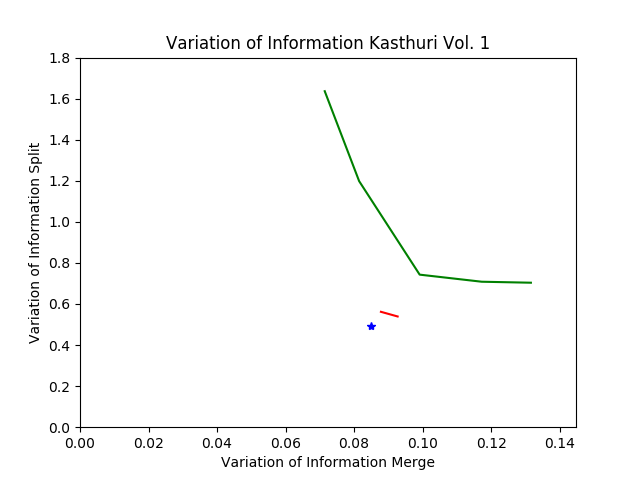
\includegraphics[width=0.45\linewidth]{./figures/variation_of_information-microns-train-600.png}
	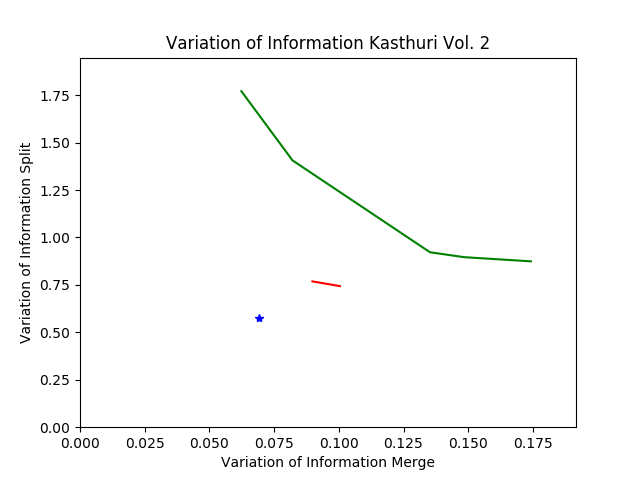
\includegraphics[width=0.45\linewidth]{./figures/variation_of_information-microns-test-600.png}
	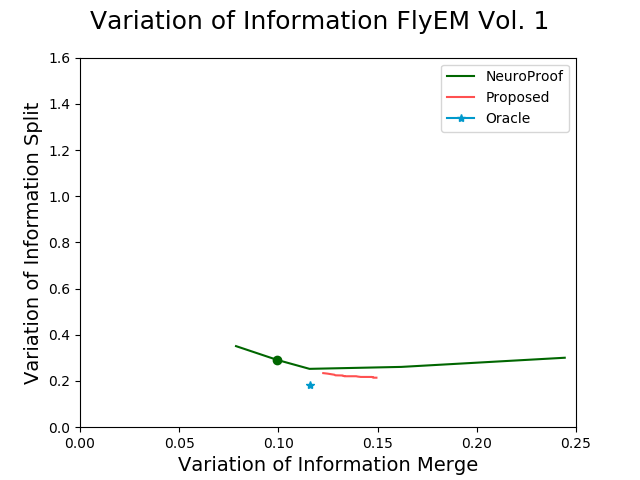
\includegraphics[width=0.45\linewidth]{./figures/variation_of_information-FlyEM-train-600.png}
	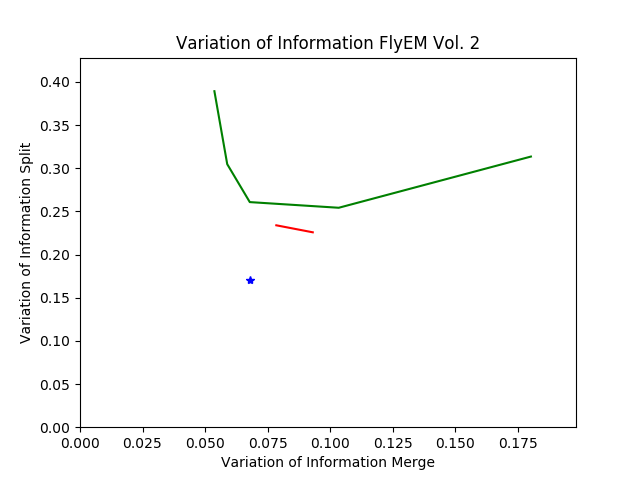
\includegraphics[width=0.45\linewidth]{./figures/variation_of_information-FlyEM-test-600.png}
	\caption{VI scores of our method (red) compared to the baseline segmentation (green) and an oracle (blue) that optimally partitions the graph based on ground truth.}
	\label{fig:variation-of-information}
\end{figure*}

%\section{Results}

\subsection{Error Metric}
\label{sec:variation-of-information}

We evaluate the performance of the different methods using the split version of variance of information (VI)~\cite{meila2003comparing}.
Given a ground truth labeling $GT$ and our automatically reconstructed segmentation $SG$, over and undersegmentation are quantified by the conditional entropy $H(GT | SG)$ and $H(SG | GT)$, respectively. Since we are measuring the entropy between two clusterings, better VI scores are closer to the origin.

\subsection{Variation of Information Results}

In Fig.~\ref{fig:variation-of-information}, we show the VI results of the pixel-based reconstructions of the Kasthuri and FlyEM data (Sec.~\ref{sec:neuroproof}) for varying thresholds of agglomeration (green). We use one of these segmentations (green circle) as out input dataset with an agglomeration threshold of 0.3 for all datasets. The results from our method are shown in red for varying X \hp{add} parameters. We show comparisons to an oracle (blue) that correctly partitions the graph from our method based on ground truth.

Our algorithm improves the accuracy of the reconstruction for every dataset, reducing the VI split score on average by \FIX{X\%} and only increasing the VI merge score by \FIX{X\%}.
Scores closer to the origin are better for this metric, and in every instance our results are below the green curve.
We see significant improvements on the Kasthuri datasets (VI split reduction of \FIX{X\%} and \FIX{X\%} on the training and testing datasets respectively) and more modest improvements on the FlyEM datasets (reduction of \FIX{X\%} and \FIX{X\%}). This is because the baseline segmentation algorithm for the isotropic FlyEM data (Sec.~\ref{sec:neuroproof}) performs much better, reducing the potential for improvements. It is well known that isotropic datasets are easier to segment using state-of-the-art region-based methods than anisotropic ones~\cite{plaza2014annotating}.

Fig.~\ref{fig:positive-results} shows successful merges on the Kasthuri Vol. 2 dataset. Several of these examples combine multiple consecutive segments that span the volume.
In the third example we correct the over-segmentation of a dendrite.
Fig.~\ref{fig:negative-results} shows some failure cases (red circles)
In two of these examples the algorithm correctly predicted several merges but made one error.
In the third example (blue circle) a merge error in the initial segmentation propagated to our output.
We now analyze how each major component of our method contributes to this final result.

\begin{figure}[t]
	\centering
	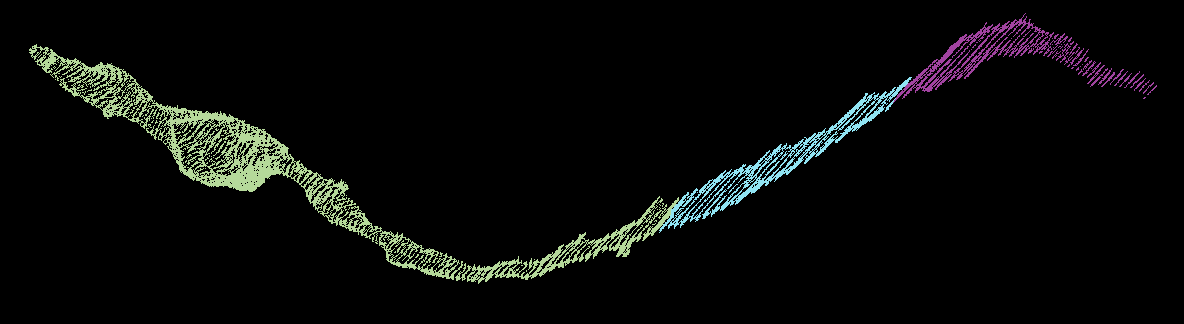
\includegraphics[width=0.85\linewidth]{./figures/multicut-correct1.png}
	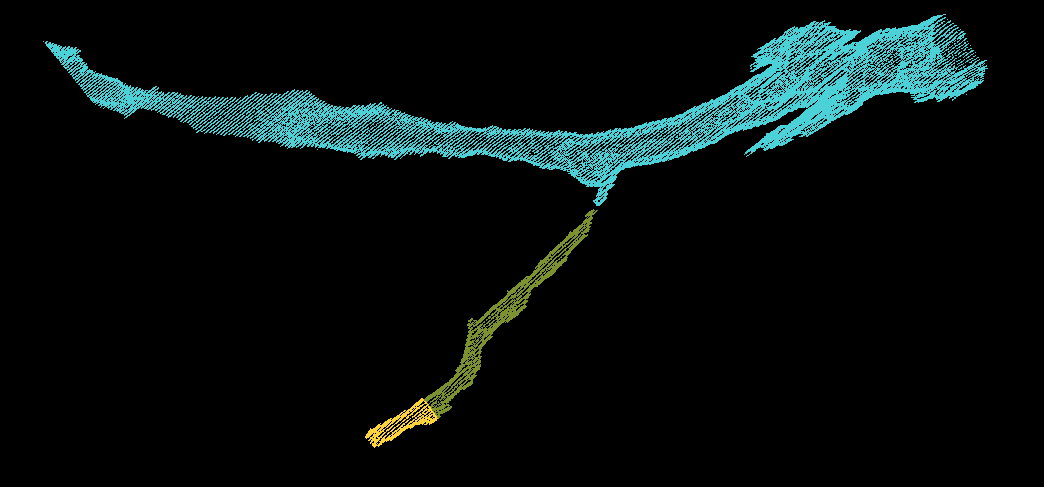
\includegraphics[width=0.85\linewidth]{./figures/multicut-correct2.png}
	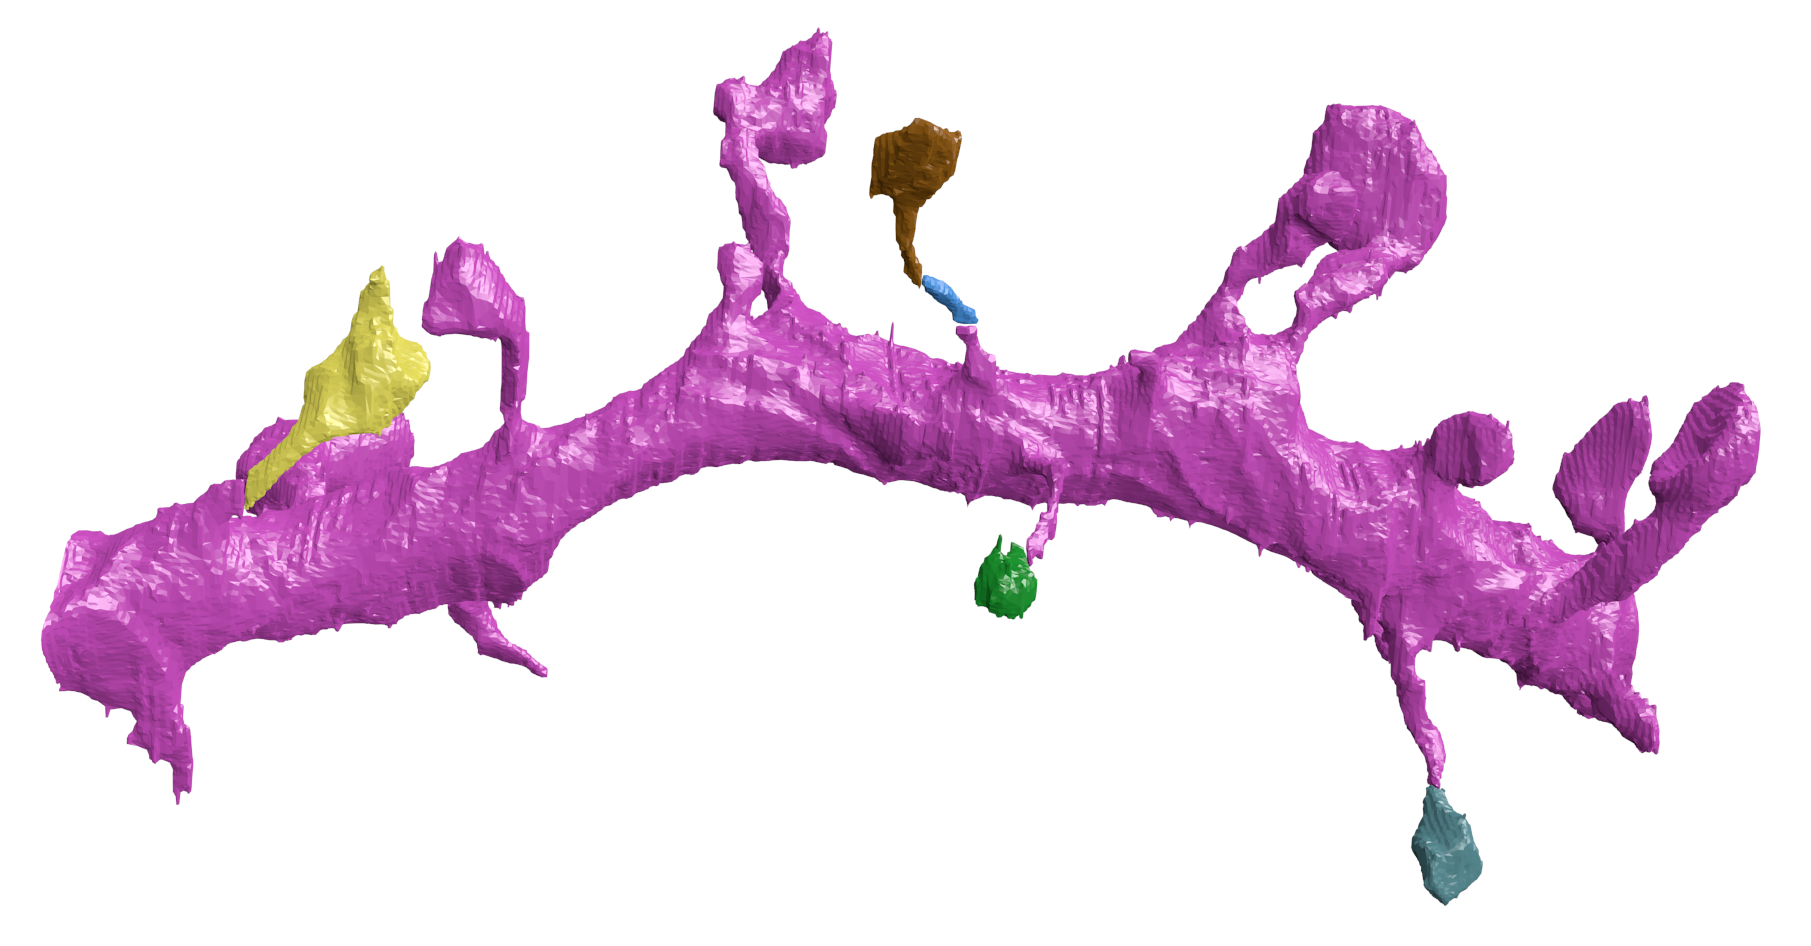
\includegraphics[width=0.85\linewidth]{./figures/multicut-correct3.png}
	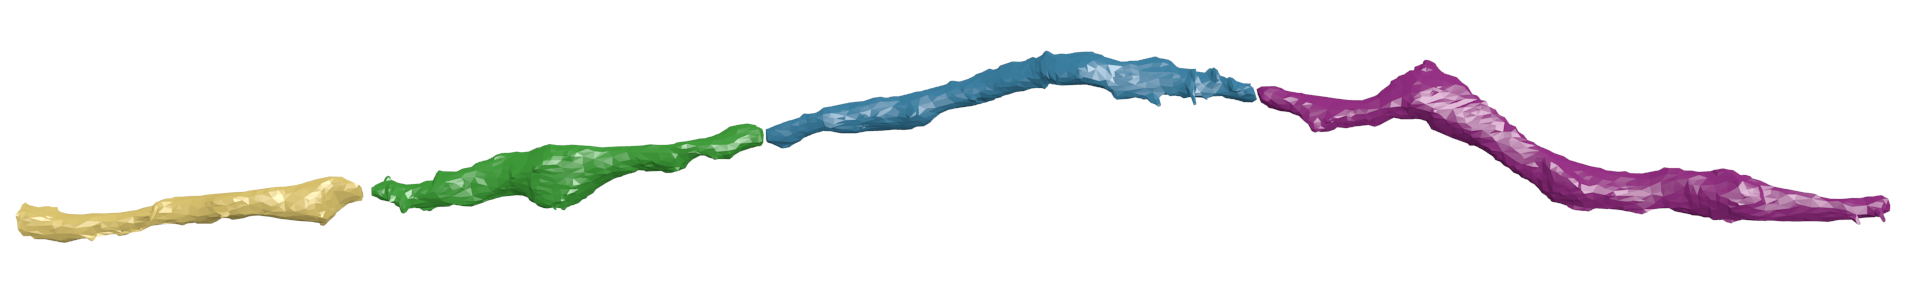
\includegraphics[width=0.85\linewidth]{./figures/multicut-correct4.png}
	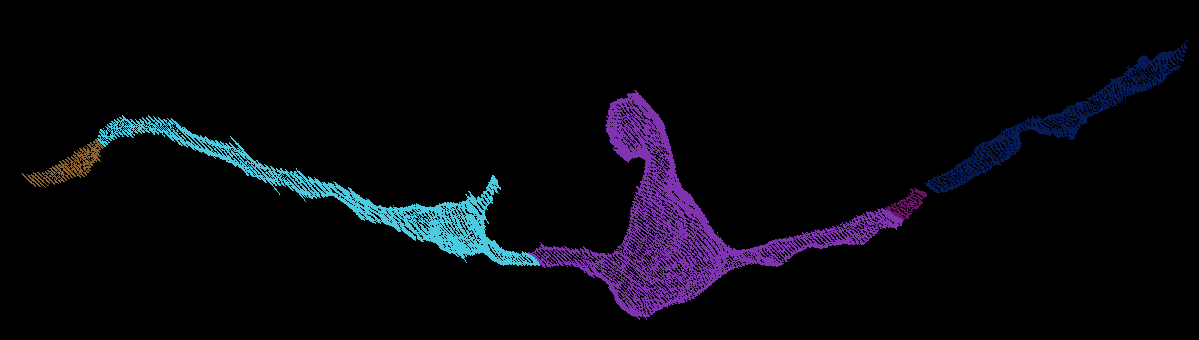
\includegraphics[width=0.85\linewidth]{./figures/multicut-correct5.png}
	\caption{Segments of neurons that were correctly merged by our method.}
	\label{fig:positive-results}
\end{figure}

\begin{figure}[t]
	\centering
	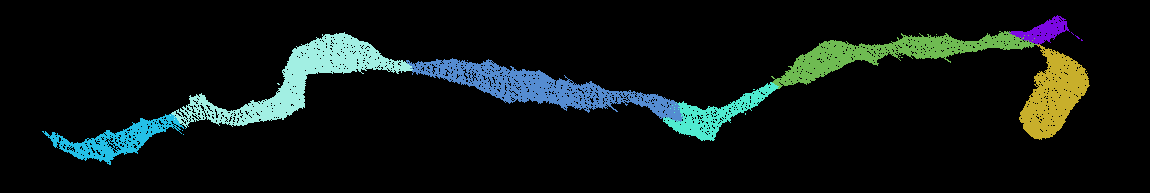
\includegraphics[width=0.85\linewidth]{./figures/multicut-incorrect1.png}
	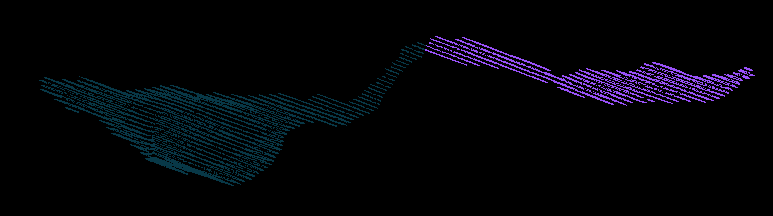
\includegraphics[width=0.85\linewidth]{./figures/multicut-incorrect2.png}
	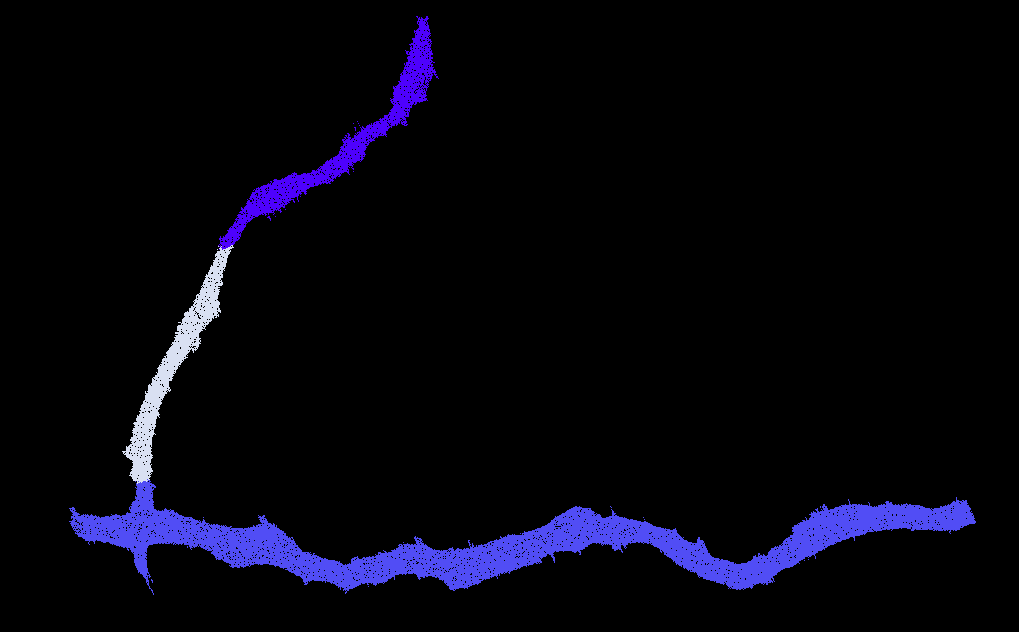
\includegraphics[width=0.85\linewidth]{./figures/multicut-incorrect3.png}
	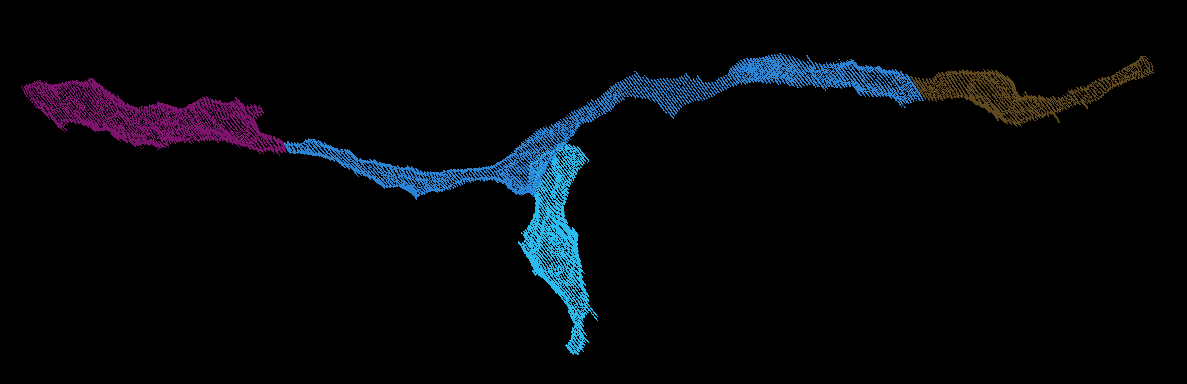
\includegraphics[width=0.85\linewidth]{./figures/multicut-incorrect4.png}
	\caption{Circles indicate areas of wrong merges by our method (red) or by the initial pixel-based segmentation (blue).}
	\label{fig:negative-results}
\end{figure}


\subsection{Graph Pruning Results}

\begin{table}
	\centering
	\small
	\begin{tabular}{c c c} \hline
		\textbf{Dataset} & \textbf{Baseline} & \textbf{After Pruning} \\ \hline
		Kasthuri Vol. 1 & 763 / 21,242 & 753 / 3,459 \\
		Kasthuri Vol. 2 & 1,010 / 26,073 & 904 / 4,327 \\
		FlyEM Vol. 1 & 269 / 14,875 & 262 / 946 \\
		FlyEM Vol. 2 & 270 / 16,808 & 285 / 768 \\ \hline
%		Kasthuri Vol. 1 & 763 / 21242 (3.47\%) & 753 / 3459 (17.88\%) \\
%		Kasthuri Vol. 2 & 1010 / 26073 (3.73\%) & 904 / 4327 (17.28\%) \\
%		FlyEM Vol. 1 & 269 / 14875 (1.78\%) & 262 / 946 (21.69\%) \\
%		FlyEM Vol. 2 & 270 / 16808 (1.58\%) & 285 / 768 (27.07\%)\\ \hline
	\end{tabular}
	\caption{The results of our graph pruning approach compared to the baseline graph with all adjacent regions. We show the number of true merge locations (e.g., 763) compared to total number of edges in the graph (e.g., 21,242) for each case.}
	\label{table:skeletonization}
\end{table}

Table \ref{table:skeletonization} shows the results of pruning the skeleton graph using the algorithm discussed in Sec.~\ref{sec:skeletonization}. This edge pruning is essential for the graph partitioning algorithm, which has a computational complexity dependence on the number of edges. The baseline algorithm considers all adjacent regions for merging. Our method removes a significant portion of these candidates while maintaining a large number of the true merge locations (e.g., 753 compared to 763). Our pruning heuristic removes at least $6\times$ the number of edges on all datasets, achieving a maximum removal rate of $20\times$.

Equally important is the number of split errors that remain after pruning. These are the locations that we want to merge to create a more accurate reconstructions. For every dataset, the number of true split errors remains constant before and after pruning. \hp{not sure what you mean}
However, since our heuristic does not enforce an adjacency constraint of two regions when constructing edges in the graph, the difference does not indicate the number of examples excluded by pruning. Fig.~\ref{fig:skeleton-results} shows an example segment with a split error (green segment) that our algorithm missed. Of the successful examples in Fig.~\ref{fig:positive-results}, the second and fourth groupings contain pairs of non-adjacent segments that were merged by our method. \hp{this paragraph needs more work to make it clearer}

\begin{figure}[h!]
	\centering
	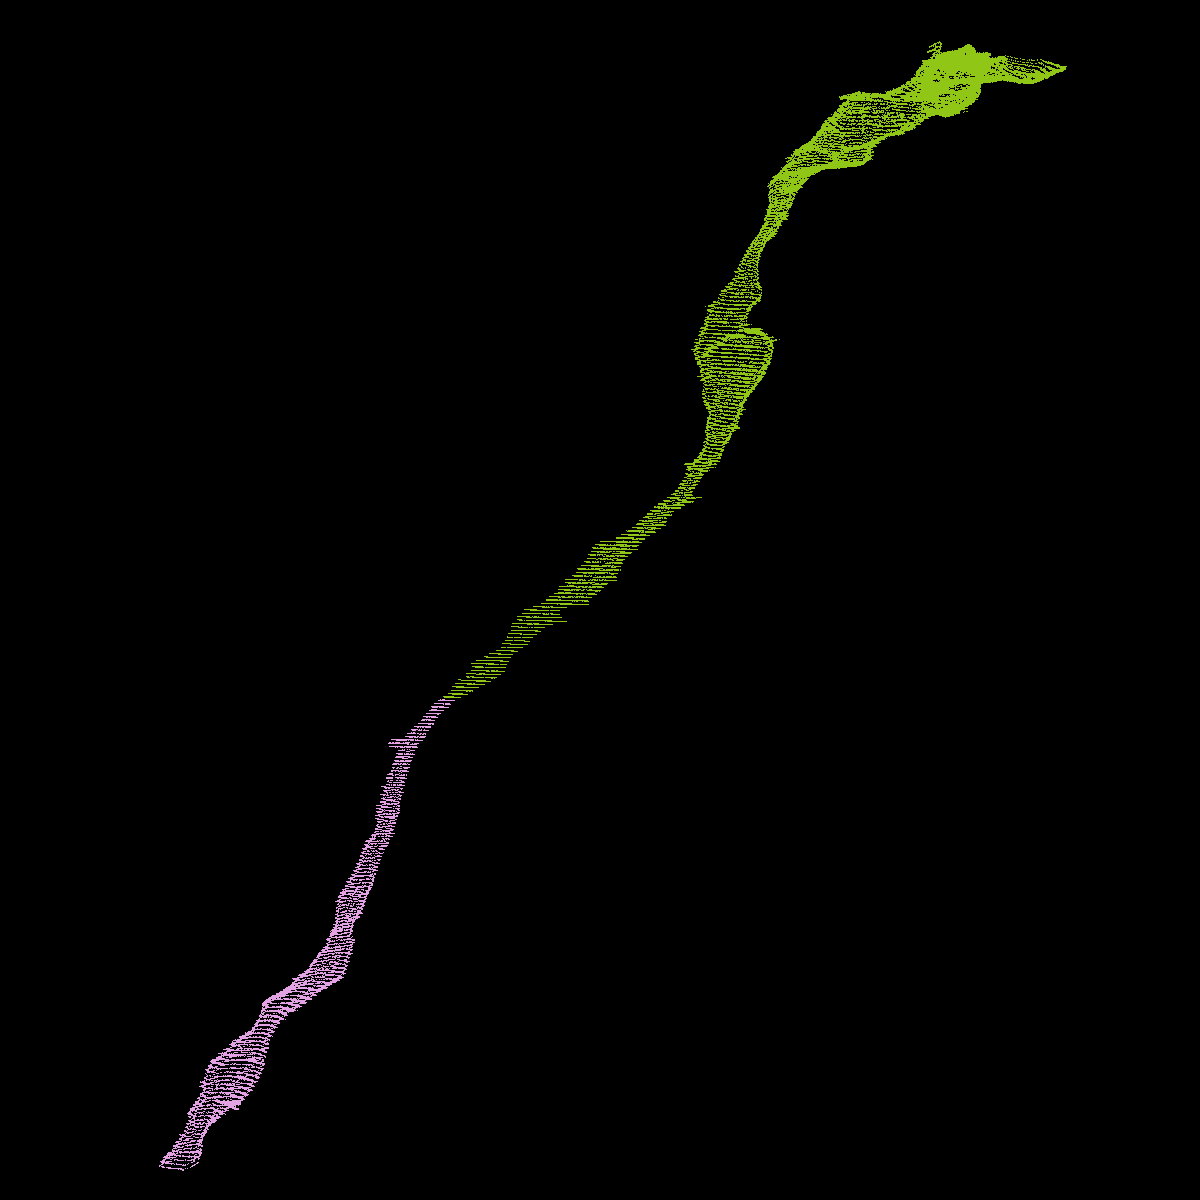
\includegraphics[width=0.85\linewidth]{./figures/merge_candidate1.png}
	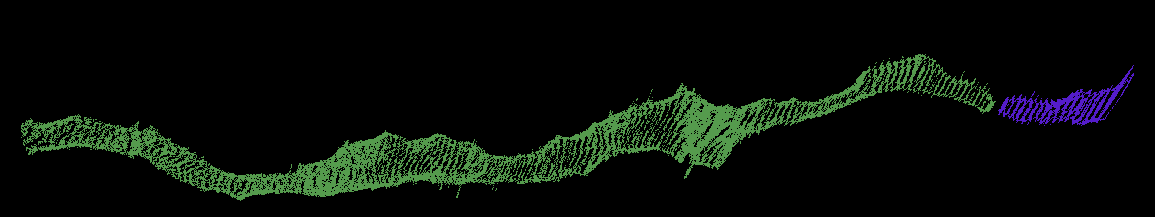
\includegraphics[width=0.85\linewidth]{./figures/merge_candidate2.png}
	\caption{Example merge candidates.}
	\label{fig:skeleton-results}
\end{figure}


\subsection{CNN Classification Results}

Figure \ref{fig:receiver-operating-characteristic} shows the receiver operating characteristic (ROC) curve of our CNN classifier for all datasets.
%We train our CNN using one of the Kasthuri volumes and test using the other three datasets.
Since our CNN only takes as input a region of the label volume we can train on  anisotropic data and test on isotropic data.
This provides a major benefit given the time-intensive task of manually generating ground truth for each dataset at various resolutions.

As shown by the ROC curve, the test results on the Kasthuri data are better than the results for FlyEM.
We believe this is in part because of the differences in the datasets (i.e., isotropy and $xy$ resolution).
To test this hypothesis, we also evaluate the performance of the FlyEM datasets when the network trains on FlyEM Vol. 1 and infers on FlyEM Vol. 2.\footnote{Since the FlyEM datasets have significantly fewer examples, we initialize the network with the weights from the Kasthuri training and have an initial learning rate of $10^{-4}$.}
The blue dotted curve in the figure shows a slight performance increase in this case. However, the improvement is minor, which led us to use the CNN trained on the anisotropic data for the rest of our experiments.

\begin{figure}
	\centering
	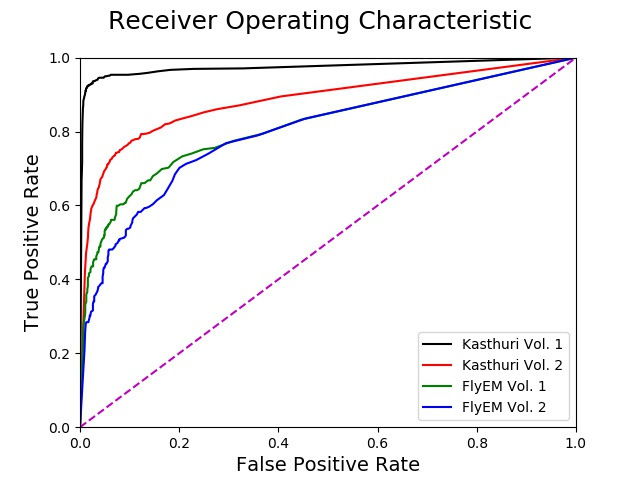
\includegraphics[width=0.95\linewidth]{./figures/receiver-operating-characteristic.jpg}
	\caption{The receiver operating characteristic (ROC) curves of our CNN for all four datasets.}
	\label{fig:receiver-operating-characteristic}
\end{figure}

\subsection{Graph Optimization Results}

The graph optimization strategy using multicut increases our accuracy over using just the CNN.
Table \ref{table:multicut} shows the changes in precision, recall, and accuracy for all four datasets compared to the CNN.
The precision increases on each dataset, although the recall decreases on all but one of the datasets.
Since it is more difficult to correct merge errors than split errors, it is often desirable to sacrifice recall for precision.
Over the three testing datasets, applying a graph-based partitioning strategy reduced the number of merge errors by \FIX{X}, \FIX{Y}, and \FIX{Z}, respectively. \hp{would be good to show the actual precision / recall numbers, too (at least in supplemental). maybe swap the ROC figure with a precision /recall figure?}

\begin{table}[h]
	\centering
	\begin{tabular}{c c c c} \hline
		\textbf{Dataset} & $\Delta$ \textbf{Precision} & $\Delta$ \textbf{Recall} & $\Delta$ \textbf{Accuracy} \\ \hline
		Kasthuri Training & +3.60\% & -0.01\% & +0.60\% \\
		Kasthuri Testing & +7.59\% & -1.77\% & +1.38\% \\
		FlyEM Vol. 1 & +2.68\% & +0.76\% & +0.66\% \\
		FlyEM Vol. 2 & +2.22\% & -1.05\% & +0.29\% \\ \hline
	\end{tabular}
	\caption{Precision, recall, and accuracy changes between CNN only and graph-optimized reconstructions for the training and three test datasets.}
	\label{table:multicut}
\end{table}
